\resizebox{\textwidth}{!}{
	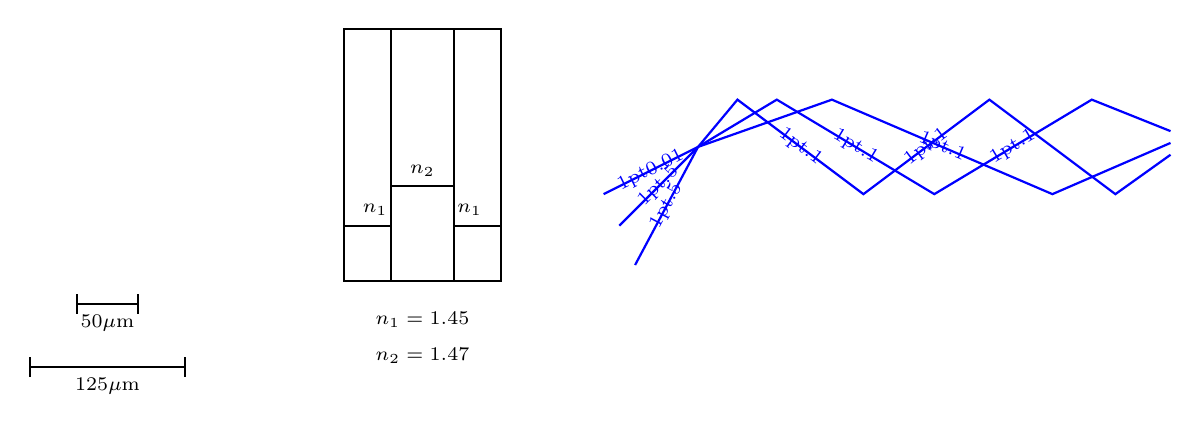
\begin{tikzpicture}[thick, every node/.style={sloped,allow upside down}, font=\scriptsize]
		\begin{scope}[yshift=1.2cm, rotate=-90]
			\doubleCylinder{.5}{.2}{3}
		\end{scope}
		\draw [|-|] (-.4, -2) -- node[below] {50$\mu$m} ++(.8, 0);

		\draw [|-|] (-1, -2.8) -- node[below] {125$\mu$m} ++(2, 0);

		\begin{scope}[xshift=4cm]
			\draw (-1, -1.7) rectangle (1, 1.5);
			\draw (-.4, -1.7) rectangle (.4, 1.5);

			\draw (-1, -1) -- (-.4, -1);
			\draw (.4, -1) -- (1, -1);
			\draw (-.4, -.5) -- (.4, -.5);

			\node at (0, -.3) {$n_2$};
			\node at (-.6, -.8) {$n_1$};
			\node at (.6, -.8) {$n_1$};

			\node at (0, -2.2) {$n_1=1.45$};
			\node at (0, -2.65) {$n_2=1.47$};

			\begin{scope}[xshift=3.5cm]
				\draw[color=blue] (-1.2,-.6) -- node {\midarrow{1pt}{0.01}} (0, 0) -- ++(1.7, .6) -- node {\midarrow{1pt}{.1}} ++(2.8, -1.2) -- ++(1.5, .65);
				\draw[color=blue] (-1,-1) -- node {\midarrow{1pt}{.5}} (0, 0) -- ++(1, .6) -- node {\midarrow{1pt}{.1}} ++(2, -1.2) -- node {\midarrow{1pt}{.1}} ++(2, 1.2) -- ++(1, -.4);
				\draw[color=blue] (-.8,-1.5) -- node {\midarrow{1pt}{.5}} (0, 0) -- ++(.5, .6) -- node {\midarrow{1pt}{.1}} ++(1.6, -1.2) -- node {\midarrow{1pt}{.1}} ++(1.6, 1.2) -- ++(1.6, -1.2) -- ++(.7, .5);
				\doubleCylinder{.7}{.3}{6}
			\end{scope}
		\end{scope}
	\end{tikzpicture}
}